% !TEX root = ../Rulebook.tex

\section{General} 
\label{sec:VRCGeneral}

Due to the Covid-19 pandemic, the RoboCup 2021 will be held online. 
Therefore, paricipating teams must provide some infrastructure to enable the TC and OC to evaluate their performance.
This is new for everyone and requires extended communication, which is why every team should join the official discord server:

https://discord.gg/z6Yn6UvhxU

Please participate in discussions and ask questions if you have any.

\section{Arena Setup} 
\label{sec:VRCArenaSetup}

As all teams will have different laboratory setups and some may not have the same resources (open space, workstations, etc. ) as others, no fixed arena design will be used for the Robocup@work 2021. We expect that this would either exclude some teams from the competitions or limit others in their test scenario design, which is why every team can design their own arena.

However, to ensure that the different robot performances can be compared using the existing scoring system (\ref{tab:Instances}), some rules are defined to encourage teams to create challenging arena designs. In addition to the basic rules described in \ref{sec:ArenaDesign}, teams are required to consider: 
  
\begin{itemize}
\item Arena size must be atleast 4m x 2m
\item The table placements should force the robot to move around the arena (not all the tables are next to each other)
\item Workstations should be accessible via multiple paths, so one of them may be blocked with obstacles (\ref{fig:vrc_arena_example} orange dots). Some space must be available for non-blocking obstacles (\ref{fig:vrc_arena_example} dark green dots).
\item Tables with the heights defined in (\ref{tab:Instances}) have to be provided (margin = 2cm). If a team doesn't have enough workstations of one type for a test, the TC may allow alternative table heights to be used (especially BTT3 and Final). This rule does not apply for the conveyor belt, the shelf and the precise placement station.
\item PPT cavities (a)-(f) (see \ref{fig:ppt_tiles}) must be provided. Teams may 3D print the cavities using the files in the leagues github. Standing objects are excluded. It must be possible to place ${N\_PLACE + 2}$ next to each other, so that atleast two decoy cavities can be used. 
\item Required arbitrary surfaces types: artificial grass, pvc floor / wood, mirror / aluminum foil, (plexi-)glass. 
These can be found in your local homedepot. (See fig. \ref{fig:vrc_obst_arbi}(b))
\item One path blocking and one small obstacle must be available both for physical objects and barriertape. (See fig. \ref{fig:vrc_obst_arbi}(a))
\end{itemize}

Figure~\ref{fig:vrc_arena_example} shows one possible example of an arena configuration in a small area.
Table heights are measured in cm. 
The orange dots mark possible path blockades, while the dark green lines mark optional obstacle placements. 


\begin{figure}[h!]
\centering
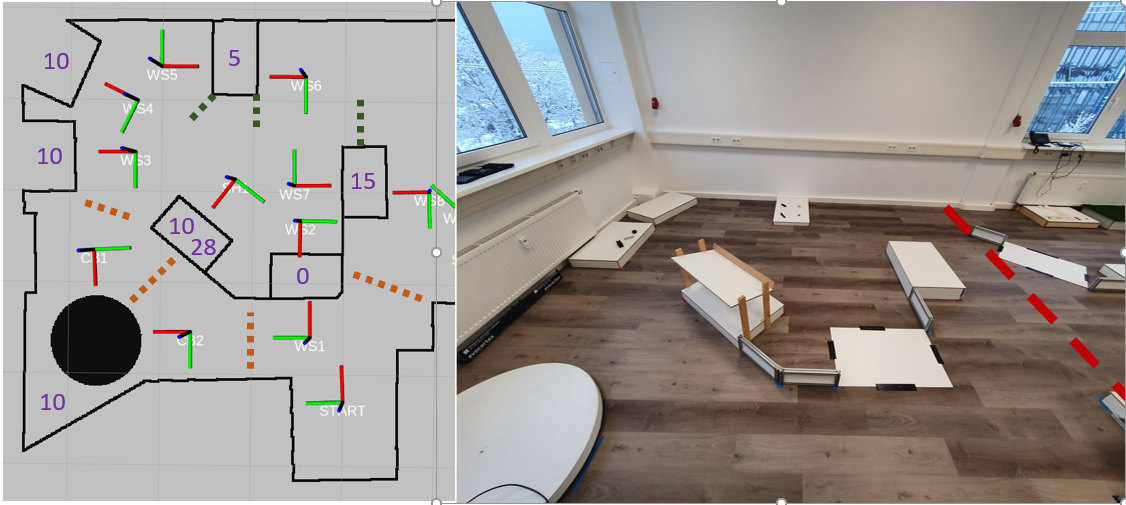
\includegraphics[width=0.9\textwidth ]{./images/vrc_arena_example.png}
\caption{Example Arena for a small VRC Setup --- Left: Annotated map - Right: Real Image }
\label{fig:vrc_arena_example}
\end{figure}

\begin{figure} [h!]
\begin{center}
\subfloat[Obstacle Placements]{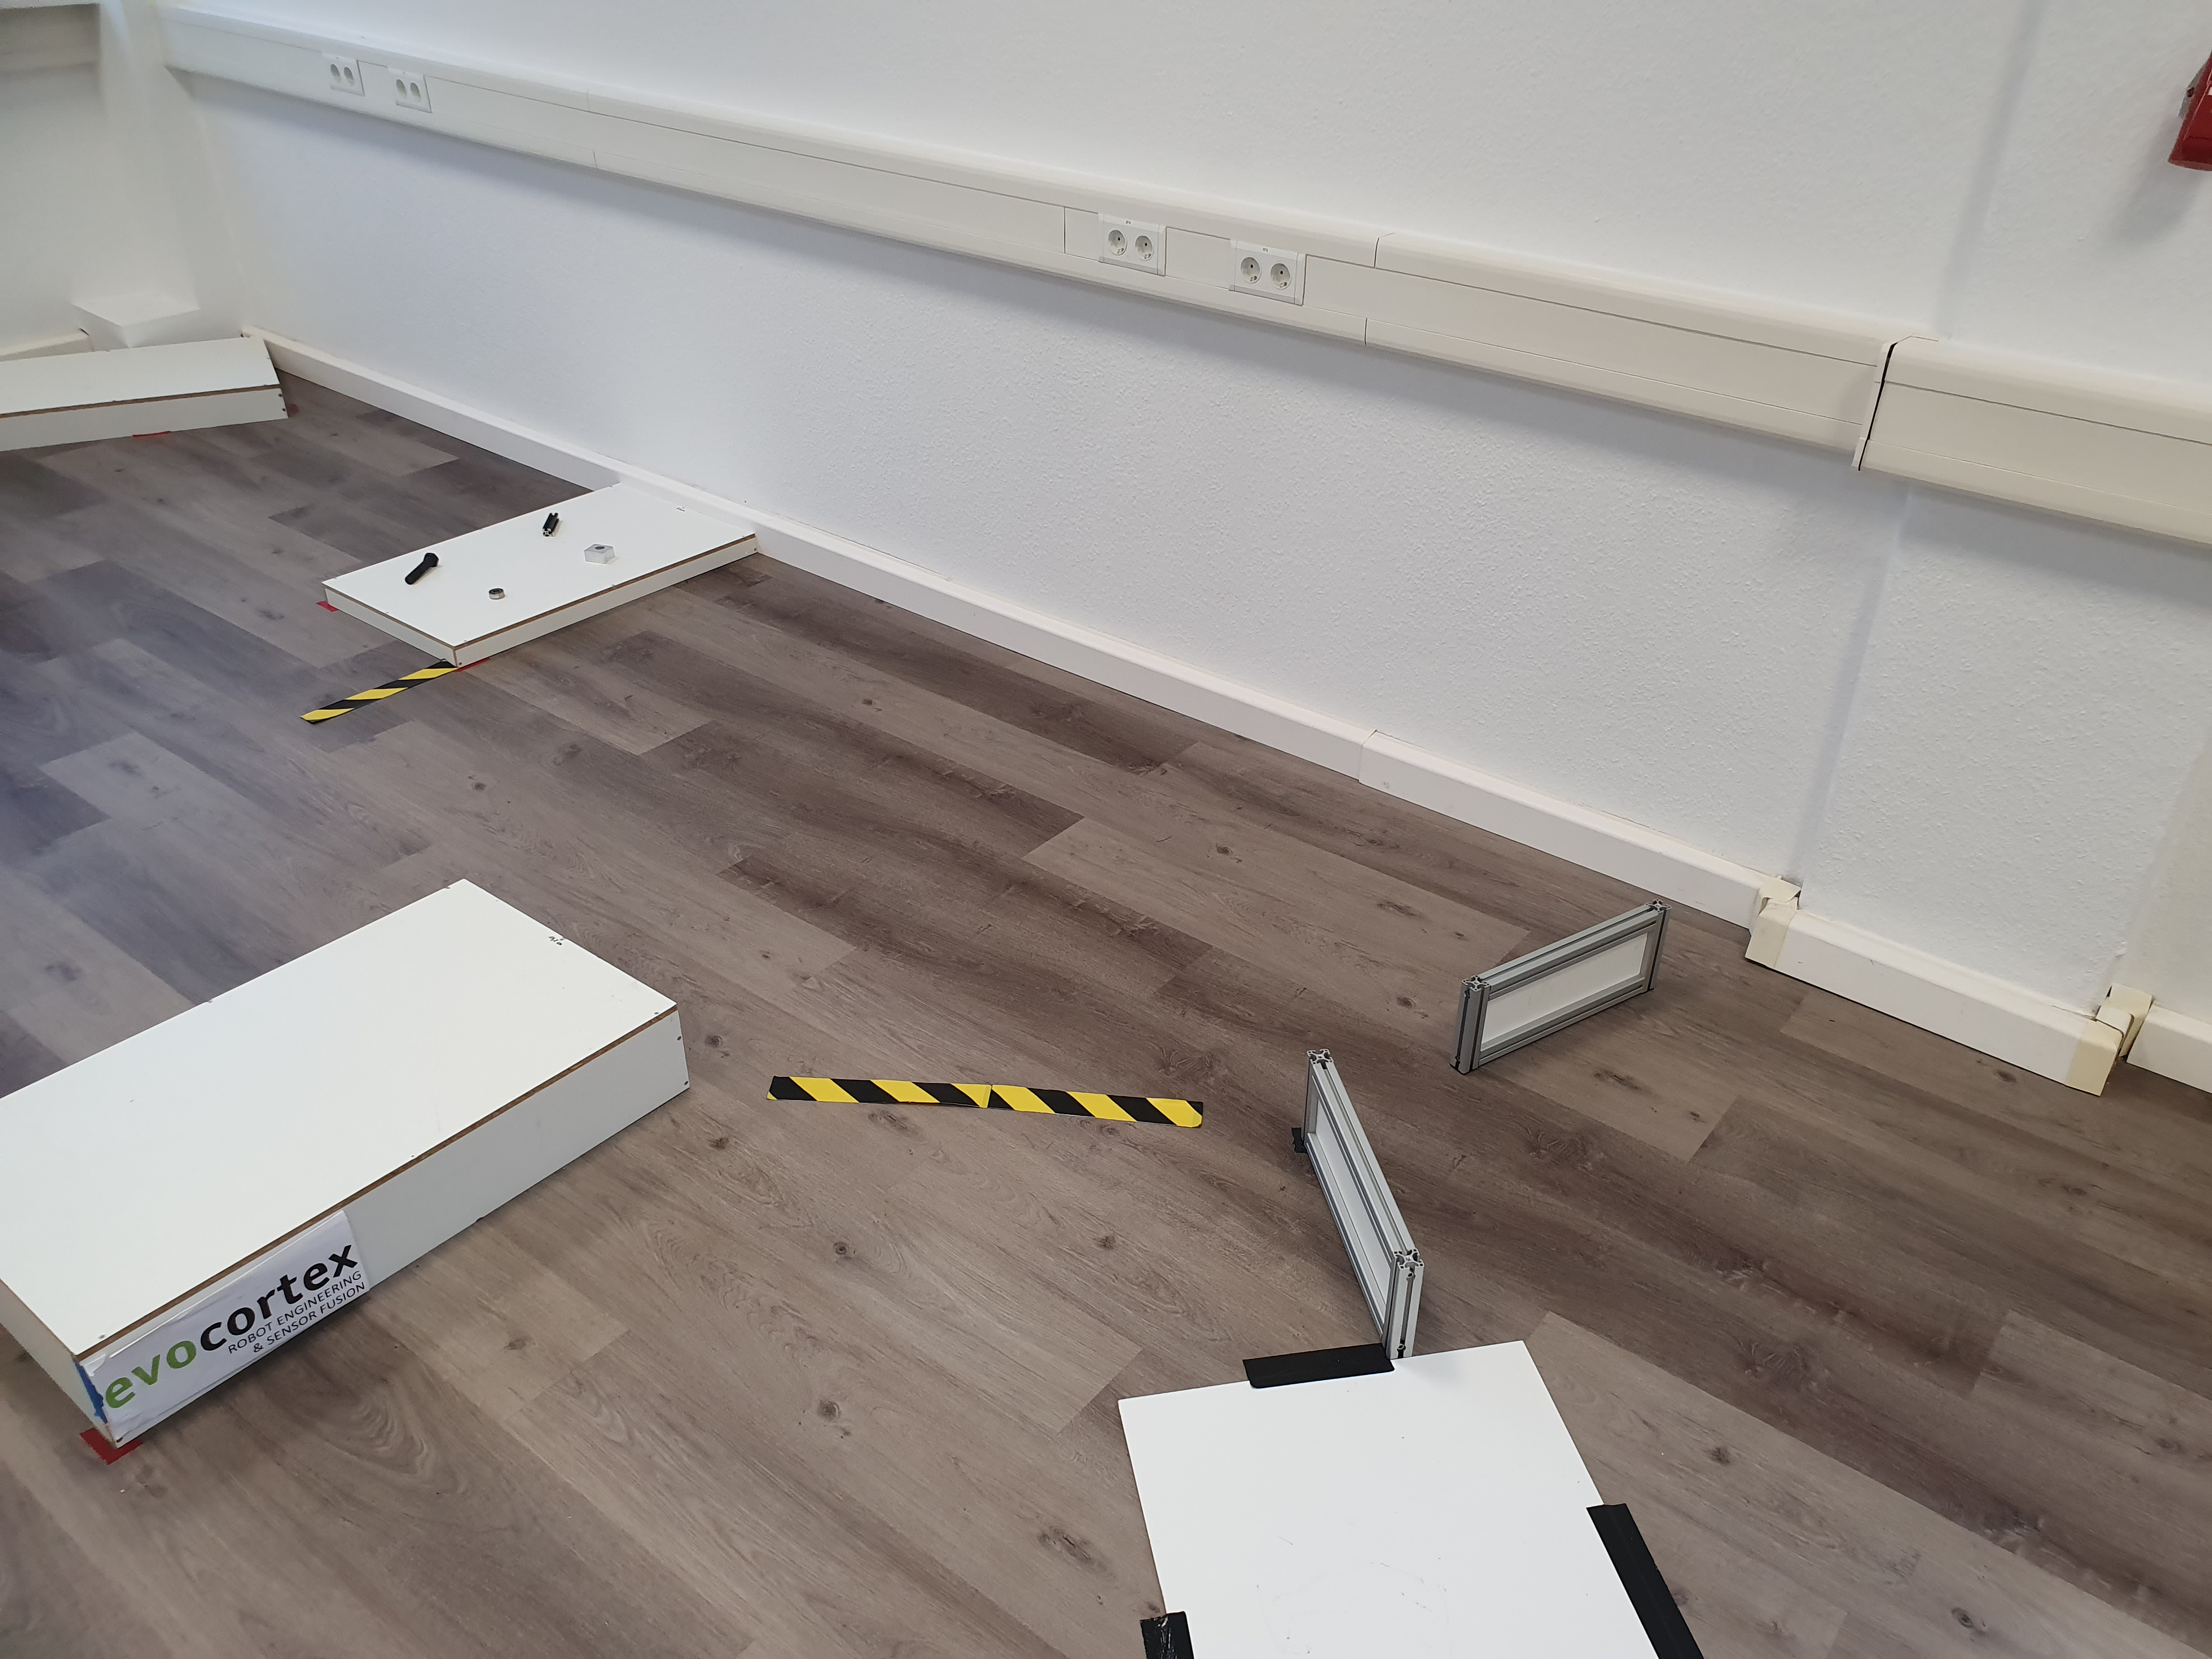
\includegraphics[height = 5cm]{./images/vrc_obstacles.jpg}} \hspace{1cm}
\subfloat[Arbitrary Surfaces]{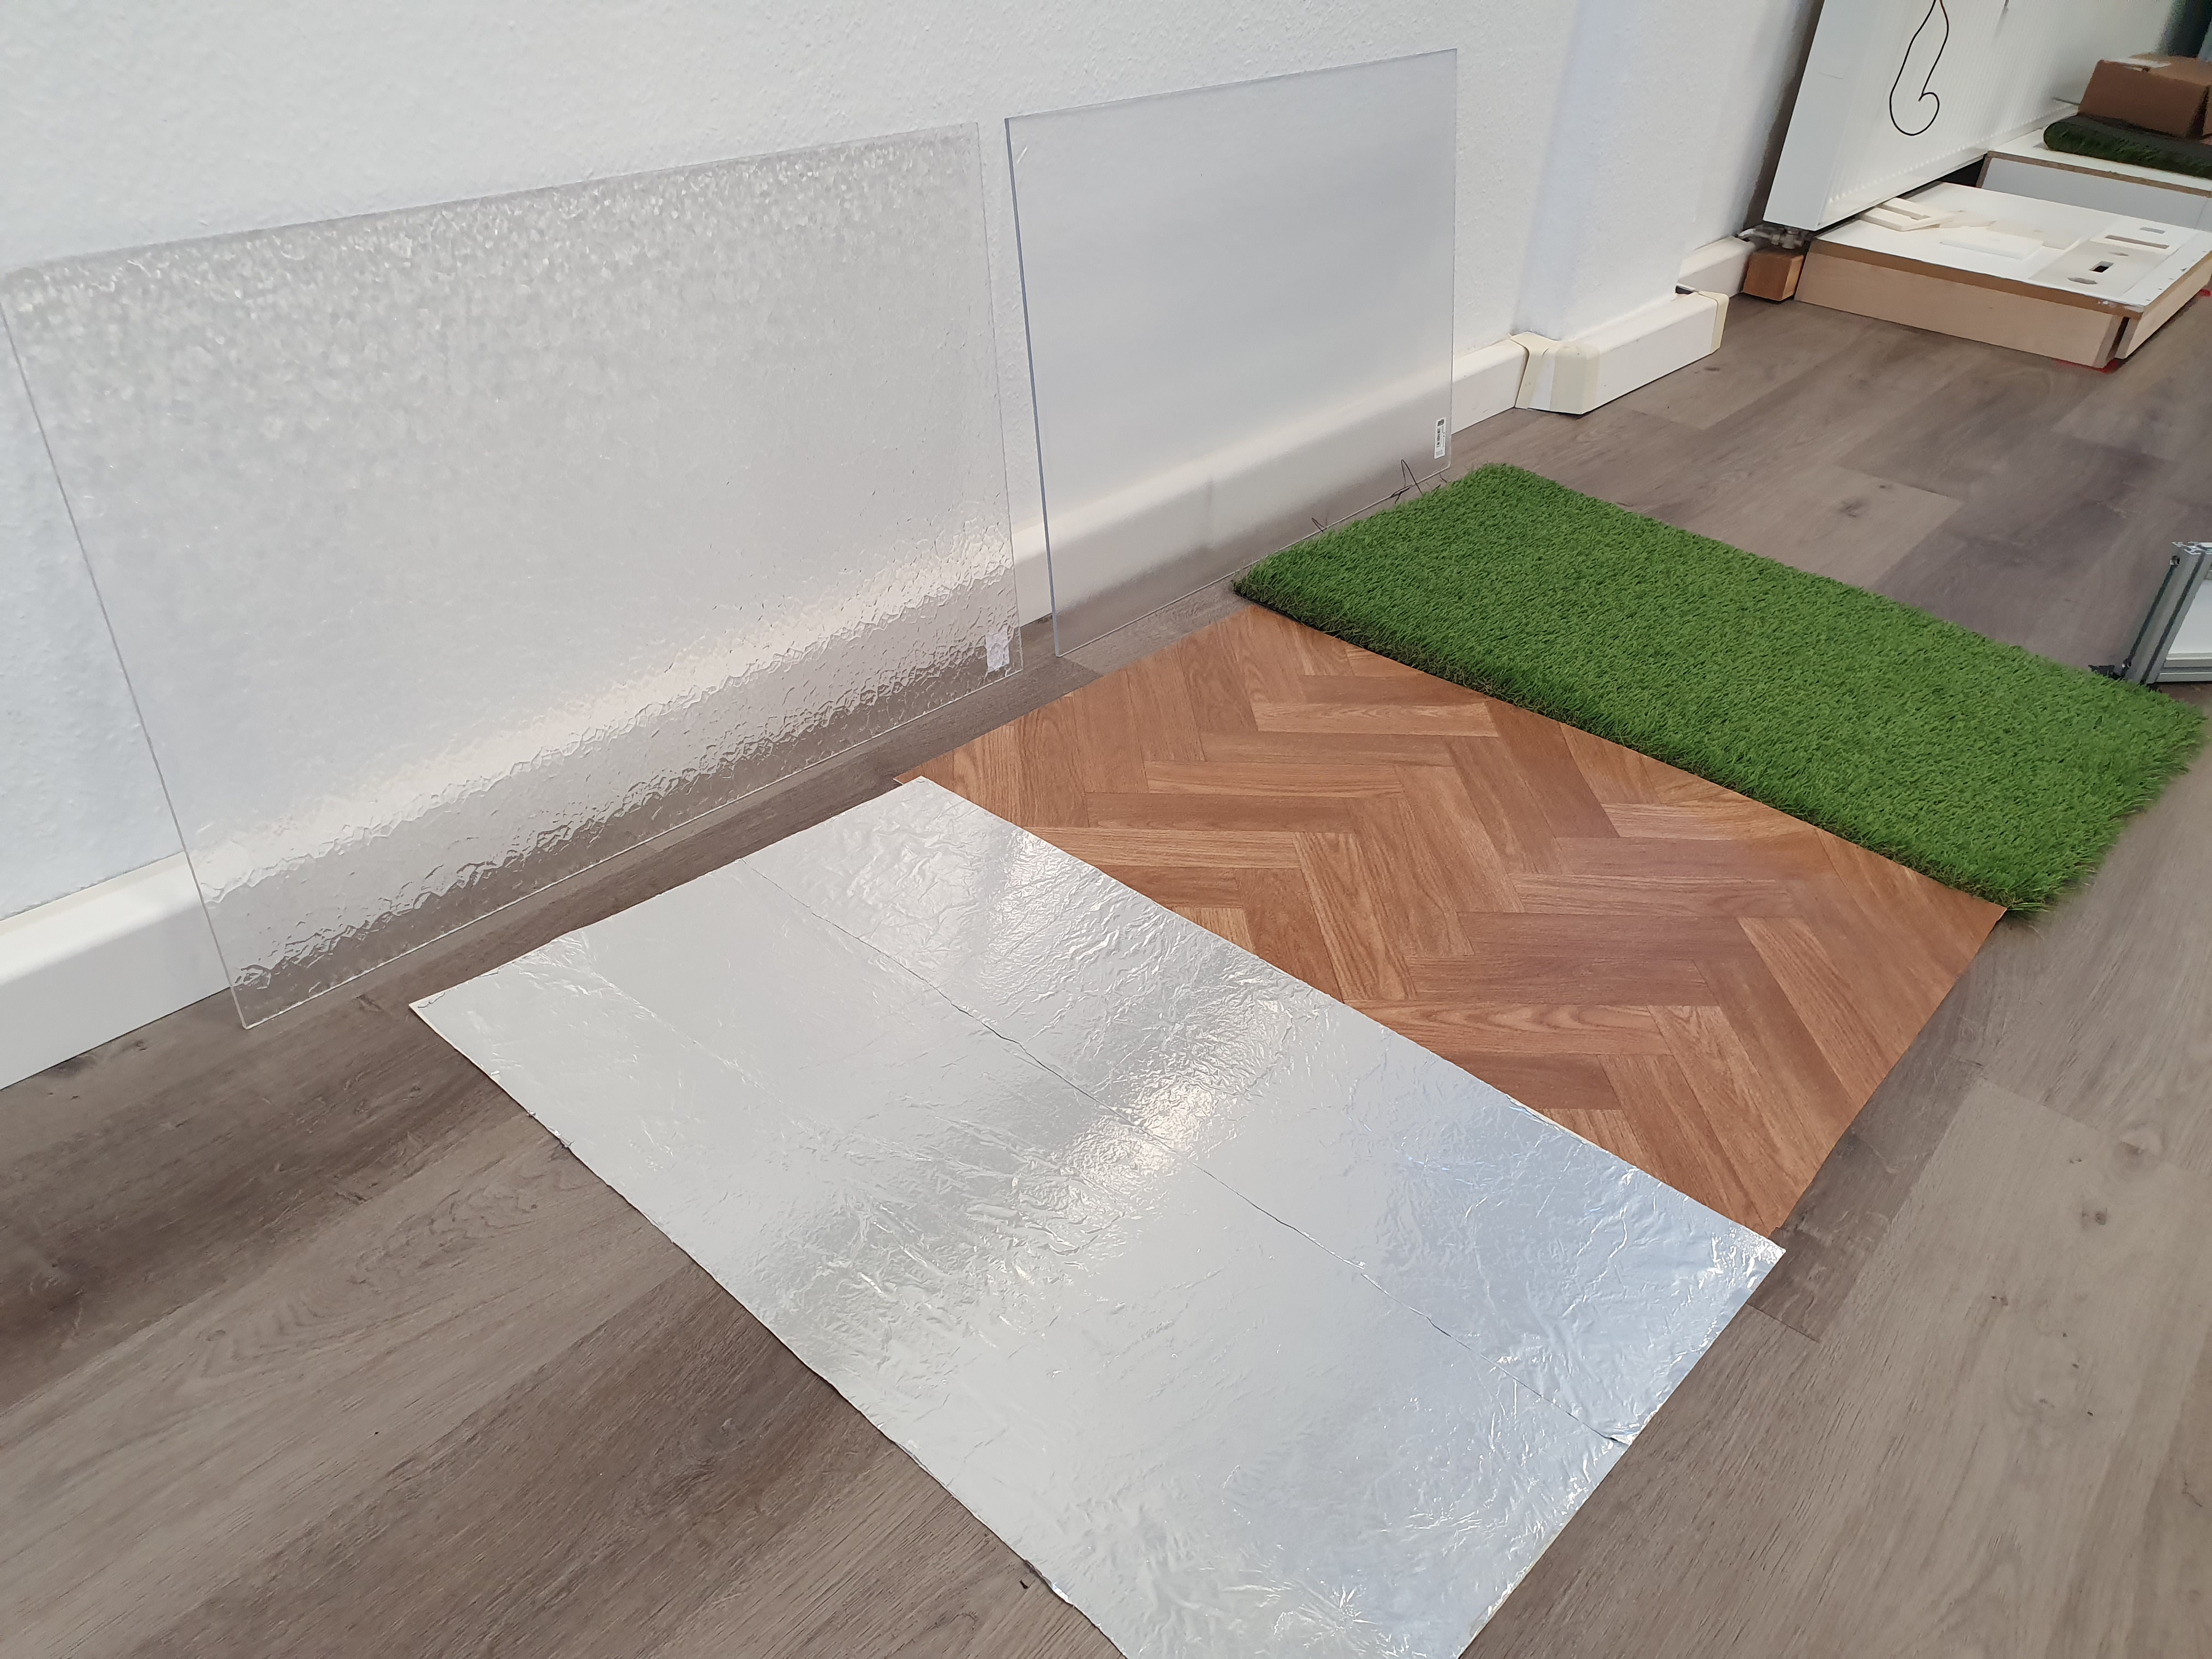
\includegraphics[height = 5cm]{./images/vrc_arbitrarys.jpg}}
\end{center}
\caption{Example obstacle placements and arbitrary surfaces}
\label{fig:vrc_obst_arbi}
\end{figure}


To enable the committee to generate fair tasks for every team, teams must provide detailed information about their arena and object inventory \textbf{1 month} prior to the first competition day. A zip-folder containing the following data must be sent via our discord server:

\begin{itemize}
\item Atleast two images of the arena from different perspectives. If two cannot cover the whole arena, teams must provide as many as needed.
\item A map of the arena with workstations marked (name + height). Teams may use an RVIZ screenshot containing the grid (1m cell size) and the occupancy grid (your map), which may be annotated using e.g. gimp (see also \ref{fig:vrc_arena_example}).
\item A list of available workstations in their arena (height and amount).
\item Images of the available arbitrary surfaces
\item Images of the available barriertape and obstacles
\item A list of available objects and containers (amount)
\item Image of the objects and containers
\item Images of the robot (all sides)
\item Robot dimensions in meter
\item Which tests the team intends to participate in
\item Refbox launchfiles
\end{itemize}

The folder must be named VRC2021-info-TEAM-NAME and shall contain the subfolders ARENA, OBSTACLES, OBJECT, ROBOT, TESTS, REFBOX. 
File names must contain information about the data (e.g. Arena-Image-1) and must not have default names (e.g. IMG2012).

The TC will decide if the individual arenas qualify for the tests defined in \ref{tab:Instances}. 
The main requirements are already specified in \ref{sec:VRCArenaSetup}, while the table describes individual task requirements more precisely.
 
If an arena does not qualify, the TC must notify the team \textbf{3 weeks} before competition starts, 
briefing the team about shortcomings and possible solutions. 
The team then has \textbf{1 week} to follow the TCs advice and provide a new zip-folder.
If an arena does not qualify for a test, the TC may decide to exclude the associated team from those.
If an arena only partly qualifies (e.g. no barriertape available), score adjustments can be made.


\section{Camera Setup} 
\label{sec:VRCCameraSetup}

Since the referees are not present at the arena during the Virtual RoboCup, the arena and all activities of the robot must be shown via livestream. For this purpose, cameras must be able to monitor the entire arena for the referees and the cameras should be mounted at least at head height. No blind spots are allowed when streaming the arena, so that the referees can see and evaluate every activity of the robot. Furthermore, the PC used to start the runs should also be monitored with the cameras so that the referees can observe every interaction with the PC. One or more cameras can be used to stream the arena. The OC will announce the streaming software used and the maximum number of livestreams available before the competition.
\par
In addition to the cameras for the arena, there must be a person who follows the robot with a mobile camera and shows the robot's activities from close up. This allows the referees to detect even small mistakes. The person is allowed to enter the arena during the run. However, the person is not allowed to interact with the robot.
\par
A camera may also be attached to the robot to better show the robot's activities to the referees and spectators. The camera on the robot is optional.

\section{RoCKIn manipulation object set} 
\label{sec:VRCRoCKInSet}
The RoCKIn objects (see table \ref{tab:manipulation_objects_rockin}) are no longer produced and sold. Because of this, it is allowed to create these objects with a 3D printer at the Virtual RoboCup. However, the 3D printed RoCKIn objects must not be mixed with original objects. This means that the complete RoCKIn object set is either original or 3D printed. Furthermore, the 3D printed objects must have the same color. This applies only to the RoCKIn object set and not to the RoboCup@Work object set (see table \ref{tab:manipulation_objects}). The RoboCup@Work object set must not be 3D printed.


\section{Task Generation} 
\label{sec:VRCTaskGen}

The new refbox implementation, which can be found here (https://github.com/robocup-at-work/atwork-commander), 
gives great opportunity to generate individual tasks for every participating team.

We advise all teams to use and test the new refbox. Teams must send configuration files for the new refbox with their arena design, so that the TC/OC can generate tasks for their arena. The config file for the arena shall contain the workstation names and heights and the available objects for a team. Teams may contact the committee via Discord if they face problems with this.  

As normally the refbox would be provided by the OC onsite, no actual refbox will be used during the online competition.
The OC will create the tasks for the tests using the official refbox and the parameters provided by the teams. 
For each test, a single bagfile (10s) will be recorded which contains all topics published by the atwork\_commander.

Teams must be able to play a bagfile on an external computer, which is connected to the robot via WiFi.
The bagfile then must be played to start a competition. The robot should receive the task and start with the execution phase.

To prevent incompatible bagfiles during the competition, 
the OC will provide test bagfiles \textbf{2 weeks} before official competitions begin.
The working parameter and launchfiles will be saved and used to generate the specific task bagfiles for the competition.

\section{Competition Test Procedure} 
\label{sec:VRCTestExec}

\subsection{Preparation} 

Before a test begins, the OC will announce obstacle placements, object positions and arbitrary surface application to a team \textbf{10 minutes} prior to their timeslot. Teams must prepare the arena accordingly. The task bagfile will be sent out to the team \textbf{5 minutes} before their official timeslot. Note: The durations may be modified during the competitions if they show to be unsuitable.

\subsection{Test Start} 

The OC may count down before a competition (3, 2, 1, go), after which they start a timer according to the test durations in \ref{tab:Instances}. On GO command, the active team may access the keyboard of the remote pc \textbf{only} to start the bagfile. The cameraman/-woman must show that to the audience.

\subsection{Test Run} 

The audience and especially the refs watch the livestream and rate the performance. In case of a major collision or any other reason for a restart, the remote pc keyboard may be accessed to restart the robot and the bagfile. The replay of the bagfile command must be shown to the audience once again, and afterwards the keybord must not be used anymore.

\subsection{Test End} 

The run ends when the timer is up, with an optional margin of five seconds due to the possible network delay. The refs then gather and discuss their performance evaluation.  

\section{Scoring} 
\label{sec:VRCScoring}

The different arena setups make time bonuses unfair and will therefore not be given in the VRC 2021. 
The rest of the scoring will be the same as in a normal robocup scenario, with score/runtime adjustments and/or penalty points possible to compensate for missing test elements (see \ref{sec:VRCArenaSetup}). Such adjustments could be:

\begin{itemize}
\item The runtime for a test may be reduced if the arena is very small
\item If no barriertape is available, all penalty points for crossing will be applied
\item If no arbitrary surface is available, the object to pick will also be removed. 
\item No containers = no placement points given
\end{itemize}

Depending on the arena setups of all teams, these rules will be defined more precisely before the competitions begin.

\section{Technical Challenges} 
\label{sec:VRCTecCha}

The 2021 virtual robocup will focus on the main competition. No technical challenges will be performed this year. We hope that we can come back to them once we have provided a smooth experience for all teams in the normal tests. We also ask for suggestions for technical challenges for the 2022 season and forward.










